\begin{figure*}
\centering
    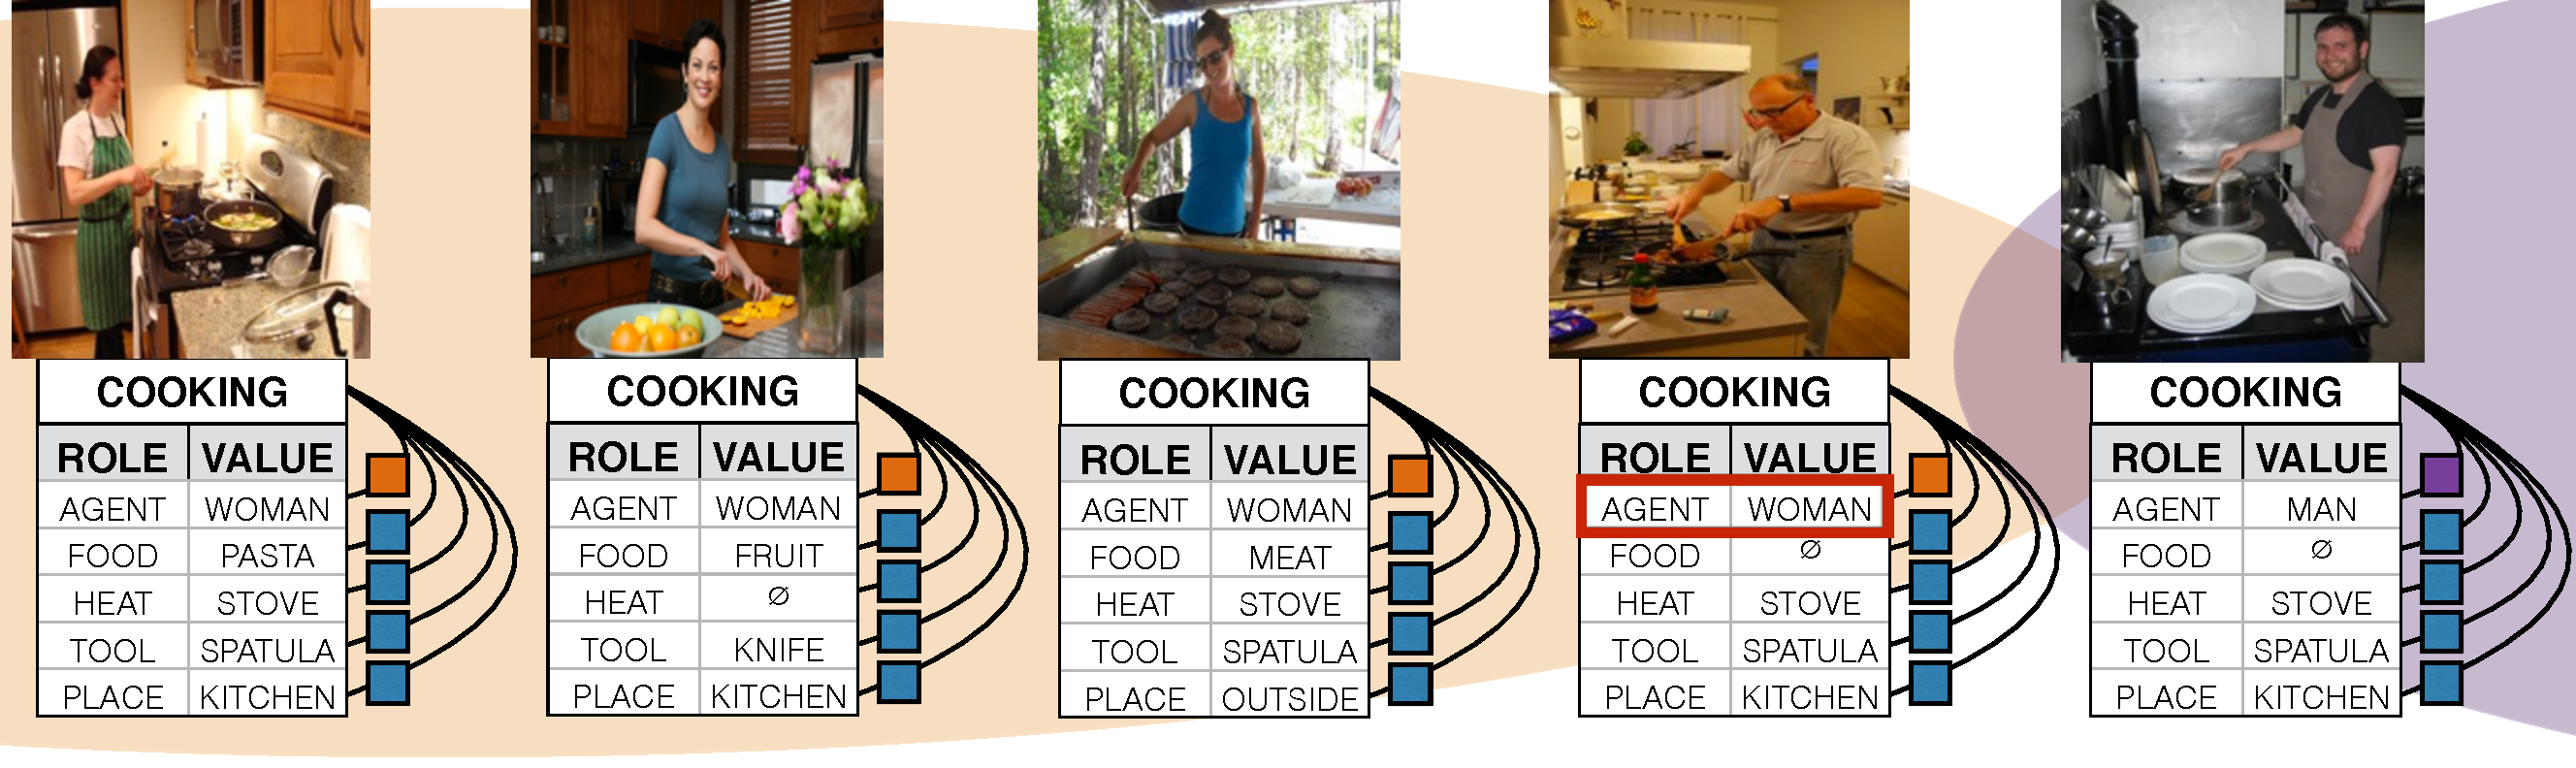
\includegraphics[width = \linewidth]{figures/pdf/bias_teaser.pdf}
\caption{ 
Five example images from the imSitu visual semantic role labeling (vSRL) dataset.
Each image is paired with a table describing a situation: the verb, \texttt{cooking}, its semantic roles, i.e \texttt{agent}, and noun values filling that role, i.e. \texttt{woman}.
In the imSitu training set, 33\% of \texttt{cooking} images have \texttt{man} in the \texttt{agent} role while the rest have \texttt{woman}.
After training a Conditional Random Field (CRF), bias is amplified: \texttt{man} fills 16\% of \texttt{agent} roles in \texttt{cooking} images.
To reduce this bias amplification our calibration method adjusts weights of CRF potentials associated with biased predictions.
After applying our methods, \texttt{man} appears in the \texttt{agent} role of 20\% of \texttt{cooking} images, reducing the bias amplification by 25\%, while keeping the CRF vSRL performance unchanged.}

\label{fig:cooking}
\end{figure*}
Visual recognition tasks involving language, such as captioning~\cite{vinyals2015show}, visual question answering~\cite{antol2015vqa}, and visual semantic role labeling~\cite{yatskar2016situation}, have emerged as avenues for expanding the diversity of information that can be recovered from images.
These tasks aim at extracting rich semantics from images and require large quantities of labeled data, predominantly retrieved from the web.
Methods often combine structured prediction and deep learning to model correlations between labels and images to make judgments that otherwise would have weak visual support.
%To model language structure and the correlation between language and vision, existing approaches combine structured prediction with deep learning. 
%in modeling the interdependencies among input and output variables.
For example, in the first image of Figure~\ref{fig:cooking}, it is possible to predict a \texttt{spatula} by considering that it is a common tool used for the activity \texttt{cooking}.
Yet such methods run the risk of discovering and exploiting societal biases present in the underlying web corpora.
%Such methods are adept at leveraging correlations between input and output variables but run the risk discovering and exploiting social biases, and, as we show later, even amplify these biases.
Without properly quantifying and reducing the reliance on such correlations, broad adoption of these models can have the inadvertent effect of magnifying stereotypes.

In this paper, we develop a general framework for quantifying bias and
study two concrete tasks, visual semantic role labeling (vSRL) and multilabel object classification (MLC). 
In vSRL, we use the imSitu formalism \cite{yatskar2016situation,yatskar2016commonly}, where the goal is to predict activities, objects and the roles those objects play within an activity.
For MLC, we use MS-COCO~\cite{lin2014microsoft,chen2015microsoft}, a recognition task covering 80 object classes.
 We use gender bias as a running example and show that both supporting datasets for these tasks are biased with respect to a gender binary\footnote{To simplify our analysis, we only consider a gender binary as perceived by annotators in the datasets. We recognize that a more fine-grained analysis would be needed for deployment in a production system. Also, note that the proposed approach can be applied to other NLP tasks and other variables such as identification with a racial or ethnic group.}.
 
Our analysis reveals that over 45\% and 37\% of verbs and objects, respectively, exhibit bias toward a gender greater than 2:1. 
For example, as seen in Figure~\ref{fig:cooking}, the \texttt{cooking} activity in imSitu is a heavily biased verb.
Furthermore, we show that after training state-of-the-art structured predictors, models amplify the existing bias, by 5.0\% for vSRL, and 3.6\% in MLC.

To mitigate the role of bias amplification when training models on biased corpora, we propose a novel constrained inference framework, called RBA, for {\bf R}educing {\bf B}ias {\bf A}mplification in predictions. Our method introduces corpus-level constraints so that gender indicators co-occur no more often together with elements of the prediction task than in the original training distribution. 
For example, as seen in Figure~\ref{fig:cooking}, we would like noun \texttt{man} to occur in the \texttt{agent} role of the \texttt{cooking} as often as it occurs in the imSitu training set when evaluating on a development set.
We combine our calibration constraint with the original structured predictor and use Lagrangian relaxation~\cite{korte08,Rush2012} to reweigh bias creating factors in the original model.
%Our method makes few assumptions about the underlying predictor beyond access to an efficient inference algorithm and is ?? some other positive statement ??. 

We evaluate our calibration method on imSitu vSRL and COCO MLC and find that in both instances, our models substantially reduce bias amplification. 
For vSRL, we reduce the average magnitude of bias amplification by 40.5\%. 
For MLC, we are able to reduce the average magnitude of bias amplification by 47.5\%. 
Overall, our calibration methods do not affect the performance of the underlying visual system, while substantially reducing the reliance of the system on socially biased correlations\footnote{Code and data are available at \url{https://github.com/uclanlp/reducingbias}}.


%Furthermore, we show that structured predictors for both of these tasks not only learn these biases but also amplify them.

%for both of these application we show that (a) 

%Consider the visual semantic role labeling task as an example, where
%the goal is to detect objects and an activity present in an image.
%When the system detects a monkey and a banana in the image, it can infer the activity {\it eating} based on correlations observed in 
%the training data.  The previous work of~\citet{yatskar2016situation} shows that 
%leveraging correlations among labels is crucial in order to achieve 
%high performance on these tasks. 


%Vision-and-language tasks, such as image captioning~\cite{vinyals2015show}, visual question answering~\cite{antol2015vqa}, and visual semantic role labeling~\cite{yatskar2016situation}, have recently drawn a significant amount of interest.
%These tasks aim at jointly learning a representation of visual content and understanding the use of language
%by bridging natural language processing and computer vision. 
%In order to model language structure and the correlation between language and 
%vision, existing approaches often apply structured prediction or deep 
%learning in modeling the interdependencies among input and output variables. 
 


%\begin{figure}
%\centering
    %\includegraphics[width = %\linewidth]{figures/cooking3.png}
%\caption{An output from a visual semantic role labeling %system. Although the 
%image clearly shows a man cooking, the system identifies %the agent as a woman. 
%This happens because the system implicitly learns the %correlation between 
%gender and the cooking activity and amplify this implicit %association present 
%in the training data.   
%}
%\label{fig:cooking}
%\end{figure}

%These models have a remarkable ability to uncover associations between visual features and language structures in an end-to-end trainable fashion, thus bypassing the need of manually defining association rules. However, this could also lead to learning associations that are stereotypical or at best unwarranted. In our work, we observed that these models often produce strongly stereotypical answers, as a byproduct of learning implicit human biases in the data. 
%Taking gender stereotypes as examples, Figure \ref{fig:cooking} illustrates the predictions for 
%a visual semantic role labeling model. Although the query image clearly depicts a {\it man} cooking, the resulting prediction suggests the agent is a 
%{\it woman}. 
%There are about twice as many images of 
%women cooking in the dataset used to train this %system~\cite{yatskar2016situation}. Moreover, we found that the model tends to 
%amplify this implicit association and make the ratio between man cooking and 
%woman cooking $1\colon 3.8$. 
% Verbs such as
%``\textit{shopping}'', ``\textit{washing}'' and ``\textit{dancing}'' 
%are biased toward ``\textit{woman}'' whereas 
%``\textit{grilling}'', ``\textit{fixing}''  and ``\textit{operating}'' 
%are biased toward ``\textit{man}''.
%We observe similar associations made by an image captioning model trained on the MS-COCO dataset~\cite{lin2014microsoft}.
%For example, when an image contains a ``snowboard'', it is very likely to 
%generate the word ``man'' in the caption, ignoring the actual gender of the 
%agent present in the image.    


%These systematic errors are rather problematic as they tend to amplify implicit associations about gender, and other demographic variables. Although error analysis suggests many errors of this type, to the best of our knowledge, there is currently no systematic way to quantify how much a learned model amplifies implicit biases.
%As a result, bias amplification is often overlooked by practitioners.  

%In this paper, we propose a general framework for quantifying implicit human 
%biases inconspicuously learned by vision-and-language models. Taking gender biases 
%\footnote{The proposed approach can be applied in other perspectives such as 
%racial biases. Also, we only consider man and woman as two gender categories 
%in this study.} as a running example, we analyze two state-of-the-art systems
%for image captioning and for visual semantic role labeling. Although we focus 
%on vision-and-language systems, the proposed framework can be generally applied in 
%analyzing other natural language processing models and intelligent systems.     

%{\bf How to debias -- 
%Calibrate the model prediction in order to remove bias. By setting up corpus-wise constraints. These constraints can be handled by LR. don't need to change infernece algorithm.  }
%{\bf Experiment results -- Highlight. number of biased verbs reduces from XXX to XXX. }.

%\jy{We further try to remove the bias caused by the models. By adding some corpus-wised constraints, we can calibrate the model prediction. For example, in imSitu, we can set the constraints for each verb to say that in the predictions, the ratio of ``man'' or ``woman'' related to this verb should be within some margin corresponding to the training ratio. All the constraints we add can be handled by the Lagrangian Relaxation algorithm~\cite{fisher1981lagrangian} without any changes in the original inference algorithm.
%The experiment result shows the efficiency of our solutions. In the semantic role labeling model, the number of biased verbs reduces from $100$ to $49$.}

%Our contribution are summarized as follows:
%\begin{compactitem}
%    \item We identify the issue of implicit human bias when modeling complex %decisions 
%		for dealing with vision-and-language problems. The proposed metric 
%		quantifies such a bias, and can be applied to various models.  
%    \item We analyze how human biases are amplified in two 
%		vision-and-language systems. The results  confirm our conjecture -- 
%		that blind statistical approaches may generate stereotypical outputs due 
%		to implicit associations.   
%    \item \jy{We add constraints to the models to avoid the amplified  gender ratio. %By adopting the Lagrangian Relaxation algorithms, we can successfully reduce the bias caused by the models without changing the original inference algorithm.}
%\end{compactitem}